\documentclass{article}[12pt]
%\usepackage{fullpage}
%\usepackage{fullpage}
\usepackage{amsmath}
\usepackage{latexsym}
\usepackage{amssymb,amsfonts}
\usepackage{graphicx}
\usepackage{graphics}
\usepackage[margin=.75in]{geometry}

\graphicspath{ {../../images/} }

\begin{document}
\newcommand{\activityname}{
  Check Mates
}
\newcommand{\subtitle}{
  Graph Theory for Grandmasters
}
\phantom{.}\hspace{-.5in}\begin{tabular}{lr}
 \begin{tabular}{l}
    
\includegraphics[width=2in]{AUExploreLogo.pdf}
 \end{tabular}
 & \hspace{.5in}
 \begin{tabular}{r}
    {\Huge \activityname}
 \end{tabular}
\end{tabular}
\thispagestyle{empty}

\noindent\hrulefill
\phantom{.}\vspace{.15in}

\noindent\textbf{Chess pieces are only allowed to move in a certain way:}

\begin{itemize}
\item A Rook (blue) is able to attack any square on the same row or column.
\begin{figure}[h]
\begin{center}
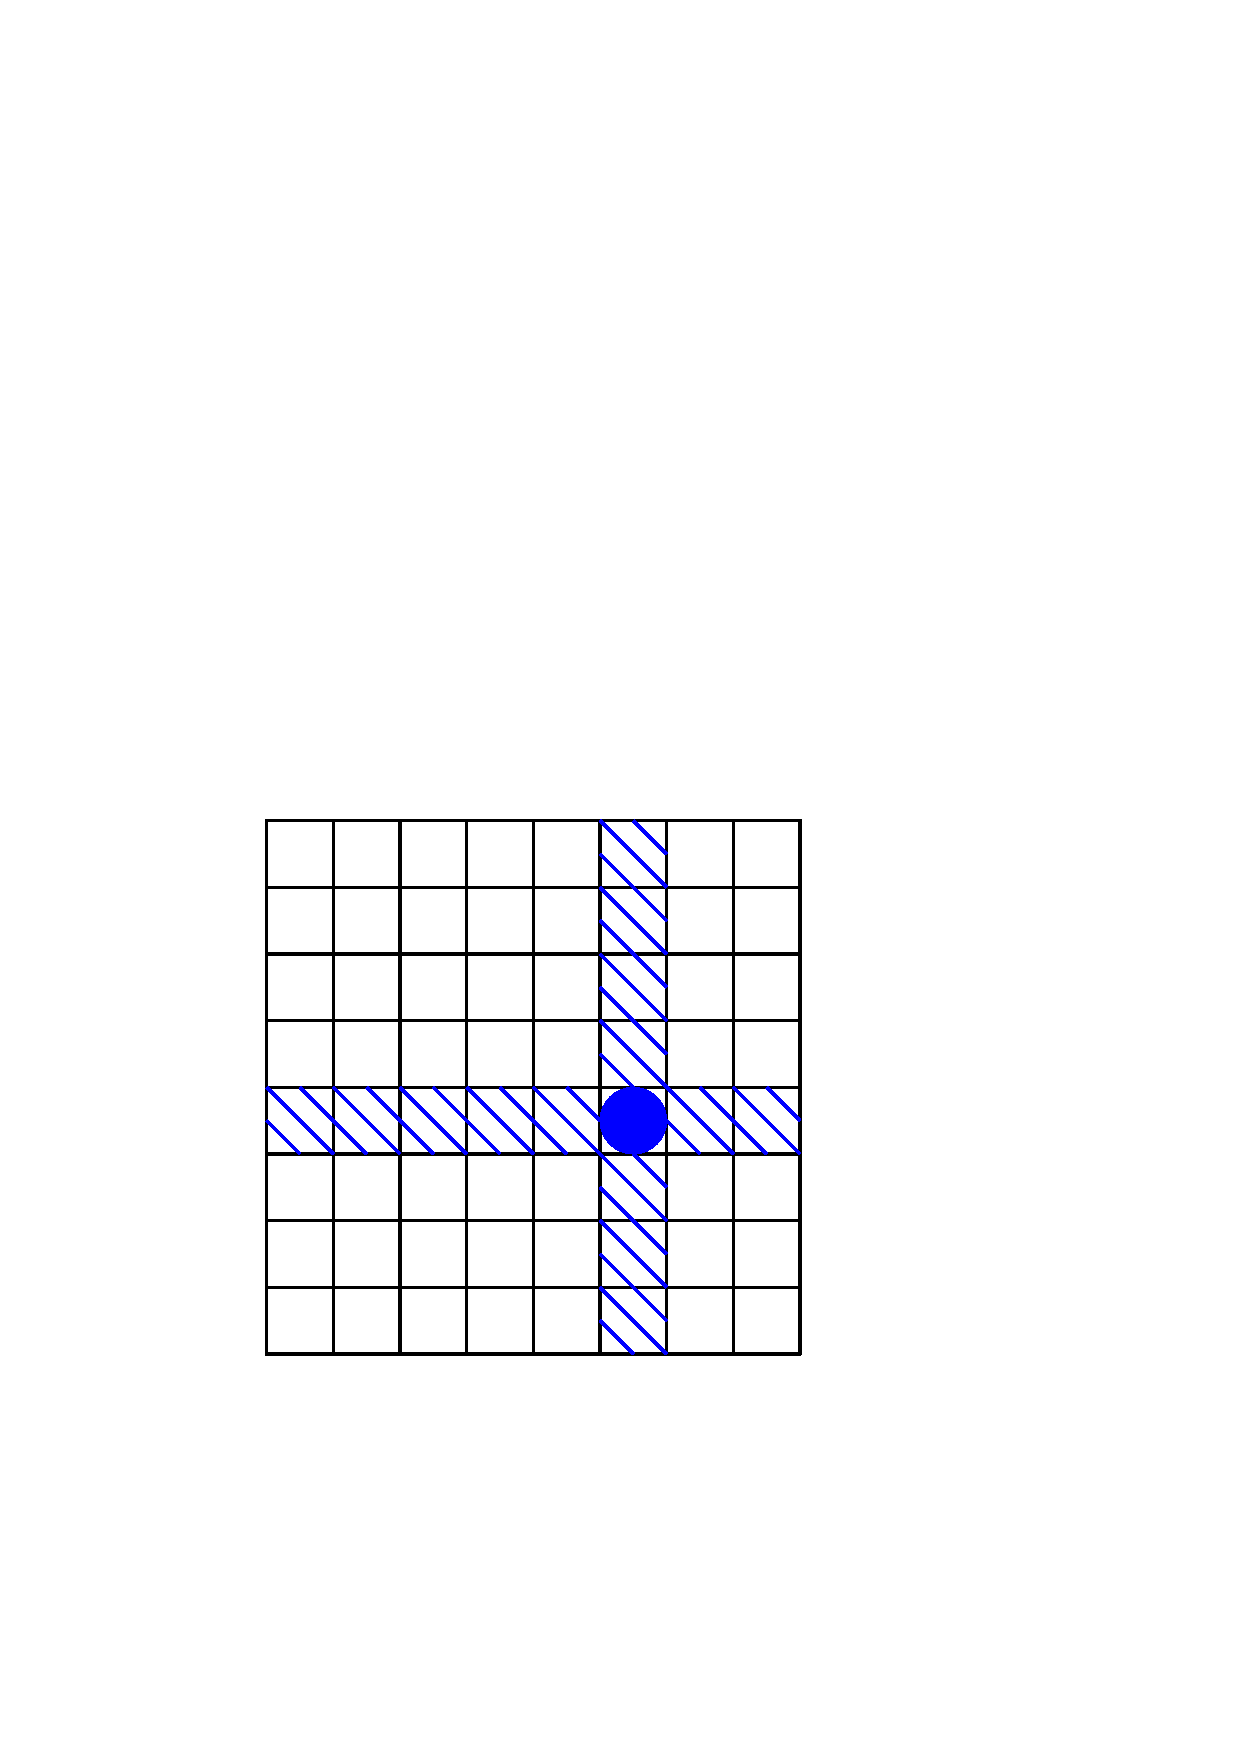
\includegraphics[width=1.3in]{RookAttack.pdf}
\end{center}
\end{figure}
\item A Bishop (orange) is able to attack any square on the same diagonal.
\begin{figure}[h]
\begin{center}
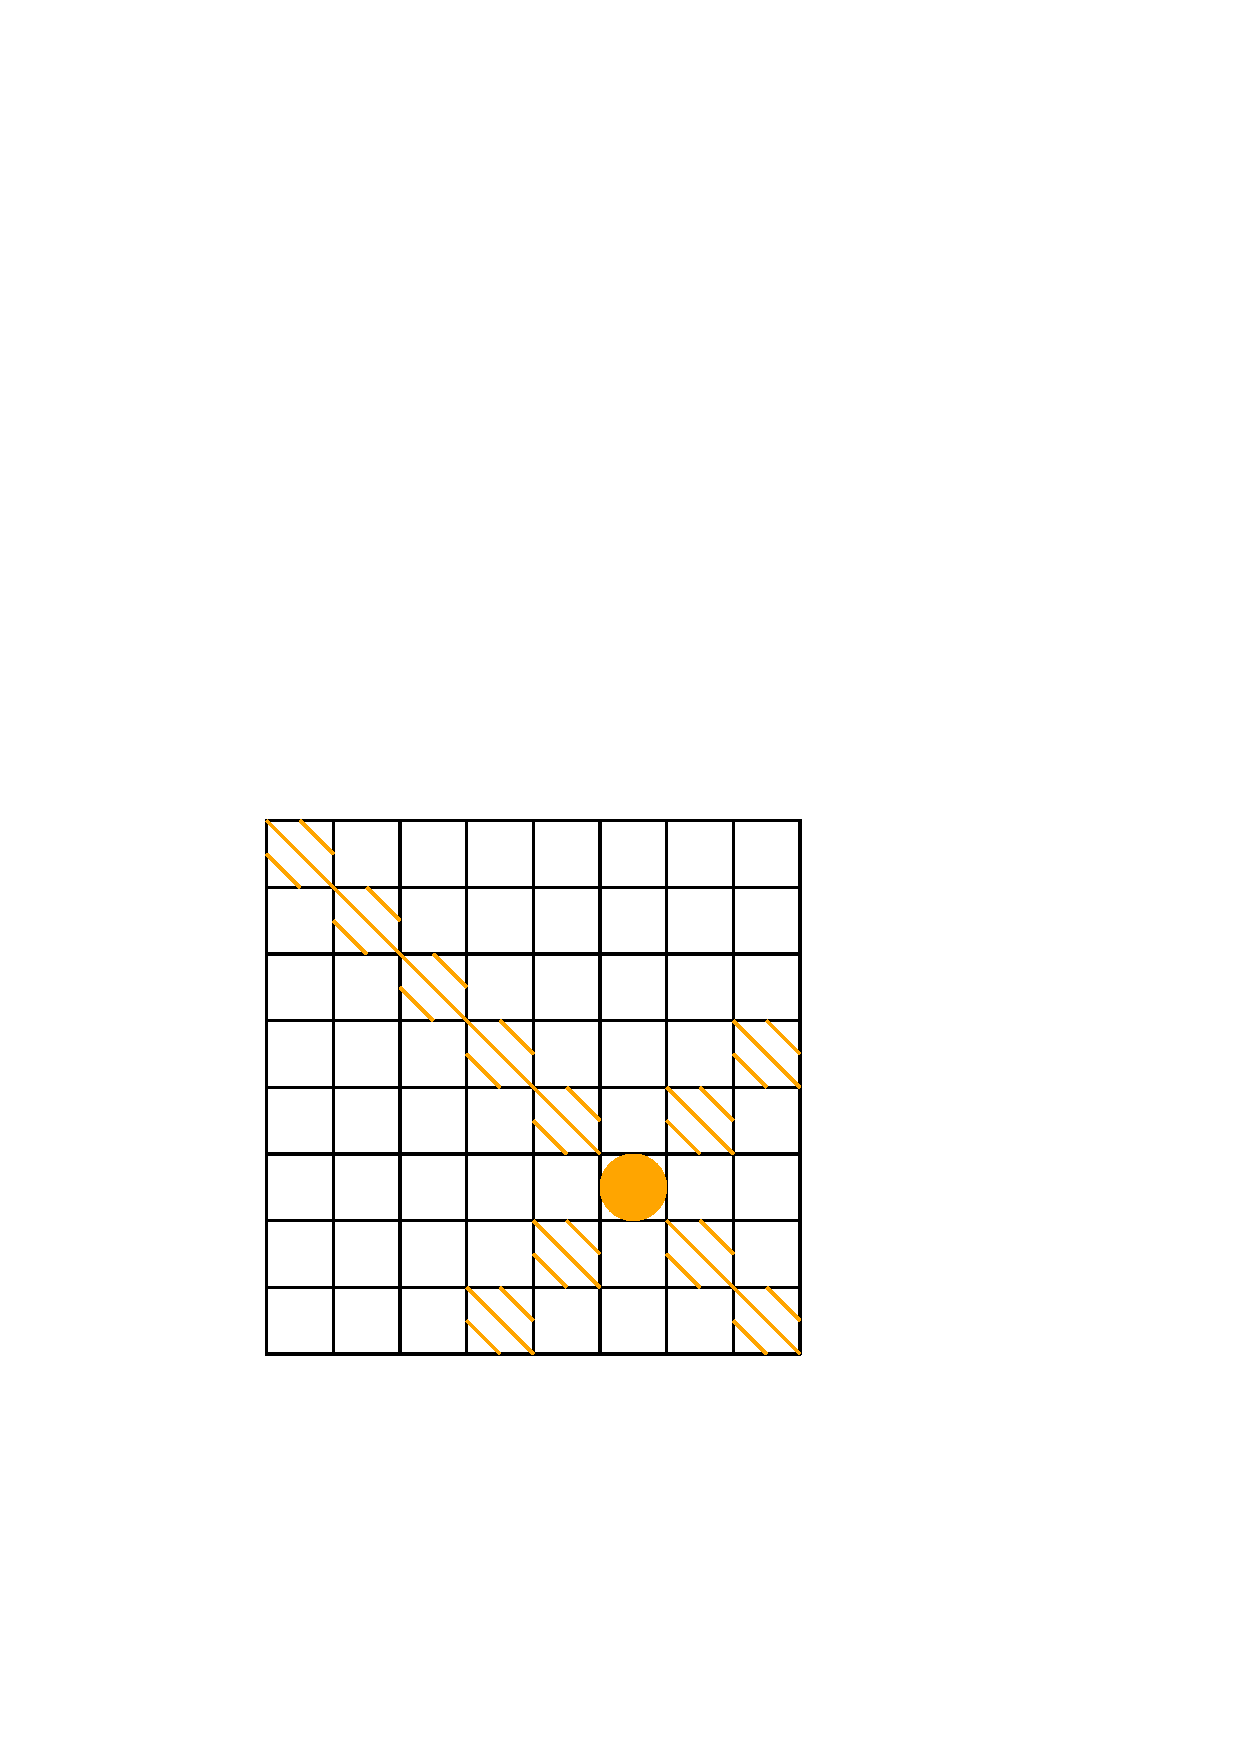
\includegraphics[width=1.3in]{BishopAttack.pdf}
\end{center}
\end{figure}
\item A Queen (green) is able to attack like a Rook OR a Bishop.
\begin{figure}[h]
\begin{center}
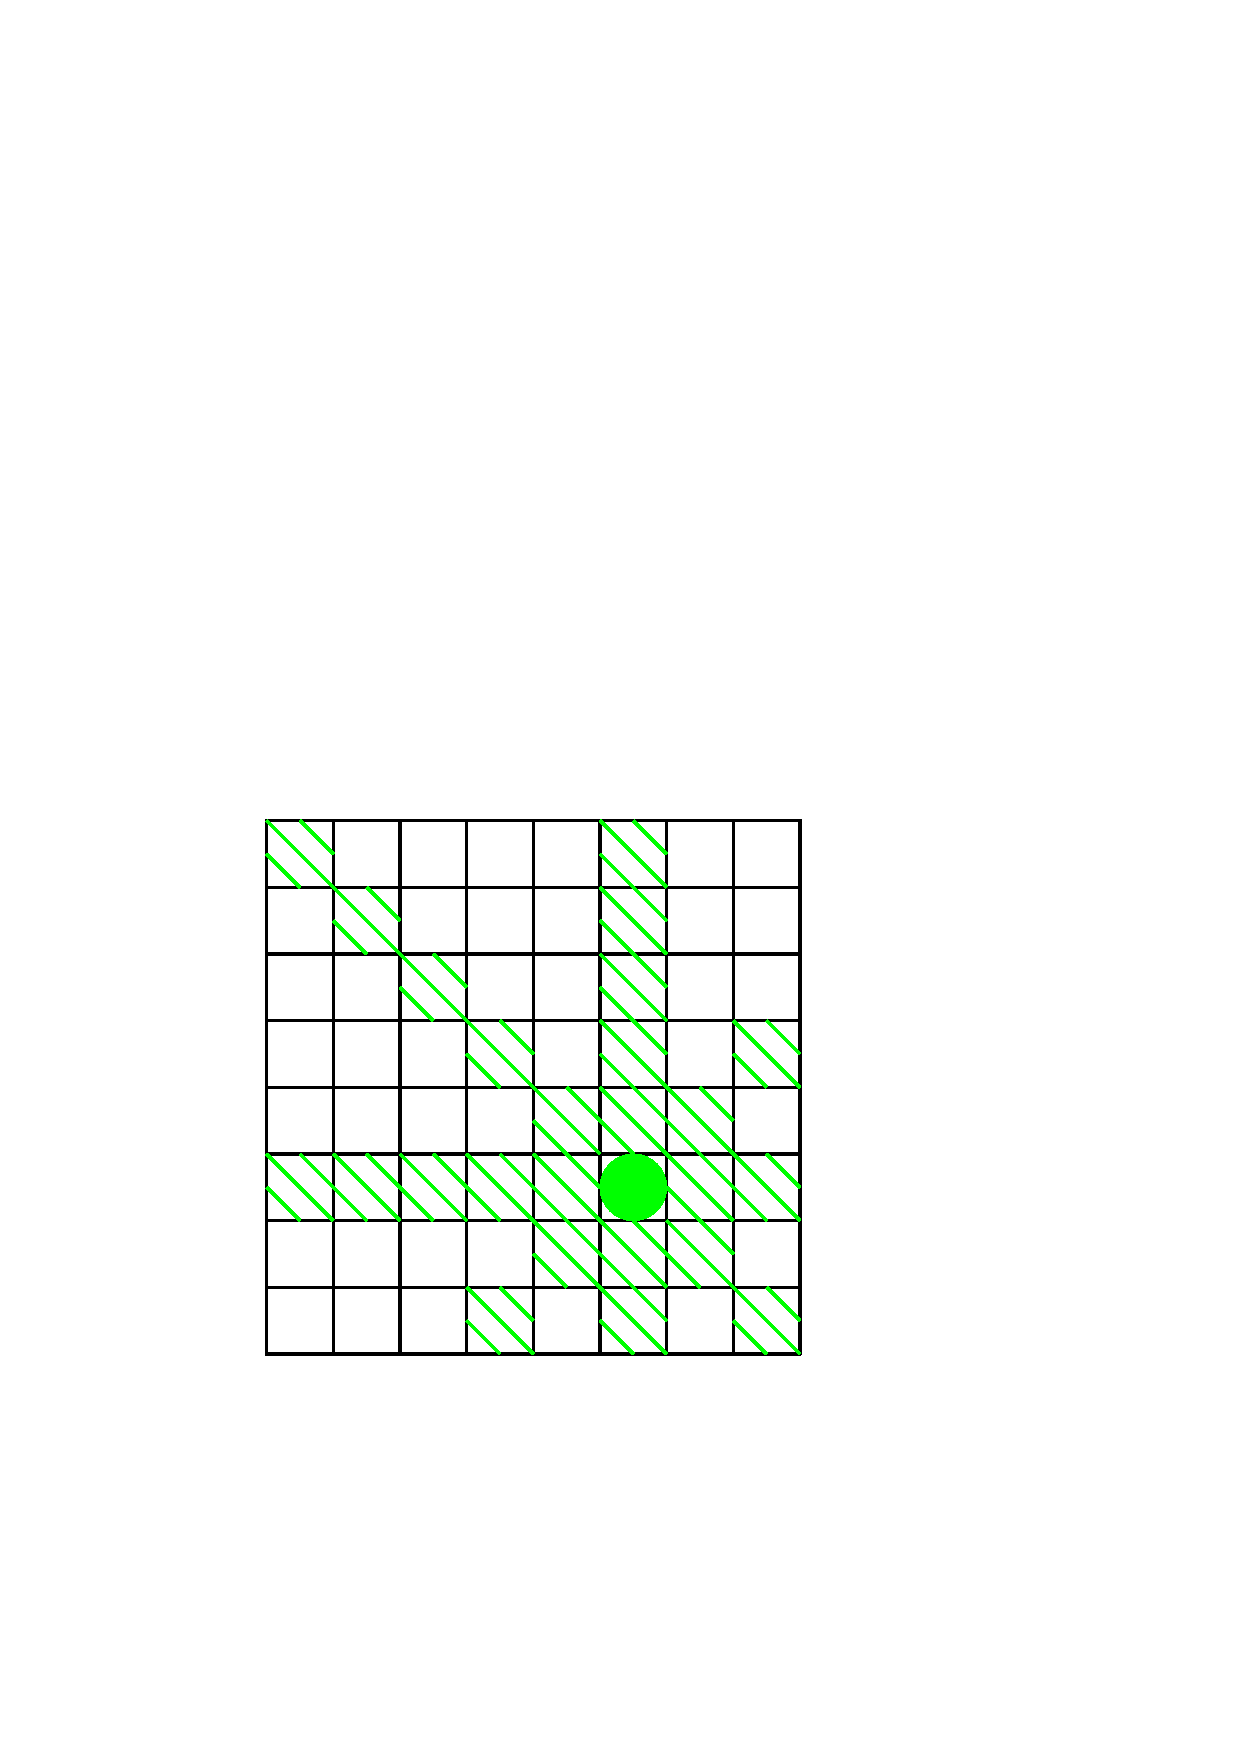
\includegraphics[width=1.3in]{QueenAttack.pdf}
\end{center}
\end{figure}
\end{itemize}

\noindent Can you fit eight Rooks on the same chessboard \textbf{such that they cannot attack one another}? What about eight Bishops? Eight \textit{Queens}?


\end{document}
